\chapter{The Cholesky Factorization and Schur Complements}
\label{ch:cholesky}

Supplementary reading:
\begin{itemize}
  \item \cite{TB} Lecture 23.
  \item \cite{Demmel} Section 2.7.1.
  \item \cite{Higham} Chapter 10.
\end{itemize}

\section{From the Normal Equations to Cholesky}

\Cref{ch:normal} reduced least squares to the normal equations $A^\ast A\vec{x} = A^\ast\vec{b}$, whose matrix $A^\ast A$ is a Gram matrix: Hermitian positive semidefinite, and positive definite when $A$ has full column rank (\Cref{thm:gram}). Four threads lead into this lecture.
\begin{itemize}
  \item \emph{Least squares by QR.} With a full QR factorization, $\norm{A\vec{x} - \vec{b}}^2 = \norm{\hat{R}\vec{x} - (Q^\ast\vec{b})_{1:n}}^2 + \norm{(Q^\ast\vec{b})_{n+1:m}}^2$. The first term is made zero by solving $\hat{R}\vec{x} = (Q^\ast\vec{b})_{1:n}$; the second does not depend on $\vec{x}$ and is the squared distance from $\vec{b}$ to $\range(A)$.
  \item \emph{The optimality condition.} $\ip{A\vec{d}}{A\vec{x}} = \ip{A\vec{d}}{\vec{b}}$ for all $\vec{d}$, i.e., the residual is orthogonal to $\range(A)$ (\Cref{thm:ls-optimality}).
  \item \emph{The normal equations.} $A^\ast A\vec{x} = A^\ast\vec{b}$ (\Cref{thm:normal}).
  \item \emph{Positive semidefinite matrices.} $M$ is Hermitian positive semidefinite if and only if $M = B^\ast B$ for some $B$ (\Cref{thm:gram}).
\end{itemize}

The factor $B$ in $M = B^\ast B$ is far from unique: $(UB)^\ast(UB) = B^\ast B$ for every unitary $U$. With so much freedom, it is natural to ask whether we can choose $B$ \emph{upper triangular}. If so, $M = R^\ast R$, and solving $M\vec{x} = \vec{c}$ takes only two triangular solves. The answer of this lecture is yes for Hermitian positive definite matrices, with no pivoting and with guaranteed stability. This is the \emph{Cholesky factorization}.

\paragraph{Conventions.} In this lecture $A \in \K^{m \times m}$ is a square matrix, unrelated to the $m \times n$ matrix of least squares. We say that $A$ is \emph{s.p.d.} if it is Hermitian positive definite; in the real case this means symmetric positive definite. Since $A$ is Hermitian, its first row is the conjugate transpose of its first column, and we write
\begin{equation}
  \label{eq:chol-block}
  A = \begin{bmatrix} \alpha & \vec{a}^\ast \\ \vec{a} & A_{22} \end{bmatrix}, \qquad \alpha = A_{11} \in \R, \quad \vec{a} = A[2{:}m, 1] \in \K^{m-1}, \quad A_{22} = A[2{:}m, 2{:}m].
\end{equation}
The product $\vec{a}\vec{a}^\ast$ is an outer product of rank one.

\section{Symmetric Elimination}

\subsection{Row Elimination from the Left}

The first step of Gaussian elimination subtracts $a_i/\alpha$ times row $1$ from row $i$, i.e., multiplies from the left by
\begin{equation}
  L_1 = \begin{bmatrix} 1 & 0 \\ -\vec{a}/\alpha & I \end{bmatrix}, \qquad
  L_1A = \begin{bmatrix} \alpha & \vec{a}^\ast \\ 0 & A_{22} - \dfrac{\vec{a}\vec{a}^\ast}{\alpha} \end{bmatrix}.
\end{equation}
The lower right block $S \doteq A_{22} - \vec{a}\vec{a}^\ast/\alpha$ is the \emph{Schur complement}, studied in \Cref{sec:schur}. Positive definiteness guarantees that the division is safe: $\alpha = \vec{e}_1^\ast A\vec{e}_1 > 0$.

\subsection{Column Elimination from the Right}

Plain LU would now continue with $S$, but then $L$ and $U$ would bear no relation to each other. To arrive at $R^\ast R$ we keep the symmetry and also multiply by $L_1^\ast$ from the right:
\begin{equation}
  L_1AL_1^\ast = \begin{bmatrix} \alpha & 0 \\ 0 & S \end{bmatrix}.
\end{equation}
Right multiplication by $L_1^\ast$ is a \emph{column} operation: column $j$ minus $\overline{a_j}/\alpha$ times column $1$. It does not change the lower right block, since the first column of $L_1A$ is zero below the diagonal. It does zero out the first row, since for $j \ge 2$
\begin{equation}
  A_{1j} - \frac{\overline{a_j}}{\alpha}\alpha = A_{1j} - \overline{A_{j1}} = 0,
\end{equation}
where the last step uses that $A$ is Hermitian. Here we see what symmetry buys: the row and the column eliminations use the same multipliers, so a single $L_1$ handles both sides.

\subsection{Normalizing by $\sqrt{\alpha}$}

It remains to normalize the pivot $\alpha$. Let $D_1 = \diag(1/\sqrt{\alpha}, 1, \dots, 1)$ and $\bar{L}_1 = D_1L_1$, which differs from $L_1$ only in its $(1, 1)$ entry. Then
\begin{equation}
  \bar{L}_1A\bar{L}_1^\ast = \begin{bmatrix} 1 & 0 \\ 0 & S \end{bmatrix}, \qquad
  \bar{L}_1^{-1} = \begin{bmatrix} 1 & 0 \\ \vec{a}/\alpha & I \end{bmatrix}\begin{bmatrix} \sqrt{\alpha} & 0 \\ 0 & I \end{bmatrix} = \begin{bmatrix} \sqrt{\alpha} & 0 \\ \vec{a}/\sqrt{\alpha} & I \end{bmatrix}.
\end{equation}
So the first column of $\bar{L}_1^{-1}$ is $A[{:}, 1]/\sqrt{\alpha}$, and
\begin{equation}
  \label{eq:chol-step}
  A = \begin{bmatrix} \sqrt{\alpha} & 0 \\ \vec{a}/\sqrt{\alpha} & I \end{bmatrix}\begin{bmatrix} 1 & 0 \\ 0 & S \end{bmatrix}\begin{bmatrix} \sqrt{\alpha} & \vec{a}^\ast/\sqrt{\alpha} \\ 0 & I \end{bmatrix}.
\end{equation}
If $S$ has a Cholesky factorization $S = L_SL_S^\ast$, substituting it into \eqref{eq:chol-step} gives
\begin{equation}
  A = LL^\ast, \qquad L = \begin{bmatrix} \sqrt{\alpha} & 0 \\ \vec{a}/\sqrt{\alpha} & L_S \end{bmatrix}.
\end{equation}
Thus the first column of the Cholesky factor is $A[{:}, 1]/\sqrt{\alpha}$, and the rest is obtained by repeating the step on $S$. Whether $S$ is again s.p.d., so that the recursion never breaks down, is the subject of \Cref{sec:chol-exists}.

\subsection{Why Divide by the Square Root of the Pivot}

Suppose we do not take square roots and simply eliminate as in LU, symmetrically on both sides. This gives
\begin{equation}
  A = \tilde{L}D\tilde{L}^\ast,
\end{equation}
where $\tilde{L}$ is unit lower triangular, $D = \diag(d_1, \dots, d_m)$ holds the pivots, and column $k$ of $\tilde{L}$ is ``the updated column $k$ divided by $d_k$''. To write this as $LL^\ast$, we split $D$ evenly between the two sides:
\begin{equation}
  A = (\tilde{L}D^{1/2})(D^{1/2}\tilde{L}^\ast) = LL^\ast, \qquad L = \tilde{L}D^{1/2}.
\end{equation}
Right multiplication by a diagonal matrix scales columns, so column $k$ of $L$ is $\sqrt{d_k}$ times ``the updated column $k$ divided by $d_k$'', i.e., ``the updated column $k$ divided by $\sqrt{d_k}$''. LU gives the whole pivot to $U$ and divides by $d_k$; Cholesky splits the pivot in half and divides by $\sqrt{d_k}$.

This requires two things. First, $D$ must be diagonal, so that $D^{1/2}$ is the entrywise square root and $\tilde{L}D^{1/2}$ is still lower triangular. Second, every $d_k$ must be positive, so that $\sqrt{d_k}$ is real, $(D^{1/2})^\ast = D^{1/2}$, and hence $(\tilde{L}D^{1/2})^\ast = D^{1/2}\tilde{L}^\ast$. If some $d_k < 0$, the square root is imaginary and the product becomes $\tilde{L}\abs{D}\tilde{L}^\ast \ne A$.

\section{The Cholesky Algorithm}

\subsection{The Right-Looking Algorithm}

Turning the derivation into an in-place algorithm, each step computes one column of $L$ and then applies the Schur complement update to the lower right block. Only the lower triangle is stored and updated.

\begin{algorithm}[H]
  \caption{Cholesky factorization, right-looking, in place (lower triangle).}
  \label{alg:chol-right}
  \begin{algorithmic}[1]
    \For{$k = 1, \dots, m$}
      \State $A_{kk} \gets \sqrt{A_{kk}}$
      \For{$i = k + 1, \dots, m$}
        \State $A_{ik} \gets A_{ik} / A_{kk}$ \Comment{column $k$ of $L$}
      \EndFor
      \For{$j = k + 1, \dots, m$}
        \For{$i = j, \dots, m$}
          \State $A_{ij} \gets A_{ij} - A_{ik}\overline{A_{jk}}$ \Comment{Schur complement update}
        \EndFor
      \EndFor
    \EndFor
  \end{algorithmic}
\end{algorithm}

Lines 2--4 divide the updated column $k$ by $\sqrt{d_k}$. In the update, both factors have already been scaled, so $A_{ik}\overline{A_{jk}}$ equals $A_{ik}\overline{A_{jk}}/d_k$ in terms of the unscaled entries, which is exactly the entry of $\vec{a}\vec{a}^\ast/\alpha$. On exit, the lower triangle of $A$ holds $L$. Note that $A_{kk}$ in line 2 is not an entry of the original matrix: after $k - 1$ updates it is the top left entry of the current Schur complement, i.e., the pivot $d_k$.

\subsection{Comparison with LU}

\begin{itemize}
  \item \emph{Normalization.} Columns are divided by the square root of the pivot, for the reason explained above.
  \item \emph{Half the work and storage.} Every Schur complement is Hermitian, so only one triangle needs to be stored and updated; the other is its conjugate transpose. The cost drops from about $\frac{2}{3}m^3$ flops for LU to about $\frac{1}{3}m^3$.
  \item \emph{No pivoting.} This is proved in \Cref{sec:chol-exists,sec:chol-errors}.
\end{itemize}

\subsection{Where Positive Definiteness Enters}

The only place where the algorithm explicitly needs positive definiteness is $\sqrt{A_{kk}}$: every updated pivot must be positive, both to get a real square root and to divide by it. Positive definiteness of $A$ directly gives only that the \emph{original} diagonal entries are positive. That every \emph{updated} pivot is positive is the content of the existence theorem below.

\begin{example}[A Symmetric Matrix That Is Not Positive Definite]
  Run \Cref{alg:chol-right} on
  \begin{equation}
    A = \begin{bmatrix} 1 & 2 \\ 2 & 1 \end{bmatrix}.
  \end{equation}
  For $k = 1$, $\sqrt{1} = 1$, the first column becomes $(1, 2)^\T$, and the update gives $A_{22} = 1 - 2 \cdot 2 = -3$. For $k = 2$, we need $\sqrt{-3}$, and the algorithm fails. Both original diagonal entries are $1$; the trouble is the updated pivot.
\end{example}

\Cref{alg:chol-right} assumes a positive definite input and does no checking; in real arithmetic, \texttt{sqrt} of a negative number returns \texttt{NaN}, which then contaminates everything after it. LAPACK's \texttt{potrf} checks whether $A_{kk} \le 0$ before taking the square root, and if so stops and reports the index at which it failed.

\subsection{Left-Looking and Up-Looking Variants}

Cholesky can be arranged to have good memory access. Comparing entries in $A = LL^\ast$ for $i \ge j$ gives
\begin{equation}
  \label{eq:chol-entries}
  L_{jj} = \sqrt{A_{jj} - \sum_{k<j}\abs{L_{jk}}^2}, \qquad L_{ij} = \frac{1}{L_{jj}}\left(A_{ij} - \sum_{k<j}L_{ik}\overline{L_{jk}}\right) \quad (i > j).
\end{equation}
Three variants evaluate these formulas with exactly the same floating-point operations and, in exact arithmetic, produce the same $L$. They differ only in the order of the three nested loops.

\begin{center}
\small
\begin{tabular}{lllll}
  \toprule
  Variant & Outer loop & Produces per step & Reads & Writes \\
  \midrule
  right-looking & $k$ & column $k$ of $L$ & column $k$ & whole trailing Schur complement \\
  left-looking & $j$ & column $j$ of $L$ & columns $1, \dots, j - 1$ & column $j$ only \\
  up-looking & $i$ & row $i$ of $L$ & rows $1, \dots, i - 1$ & row $i$ only \\
  \bottomrule
\end{tabular}
\end{center}

For one step of each variant, this gives the following picture.

\begin{center}
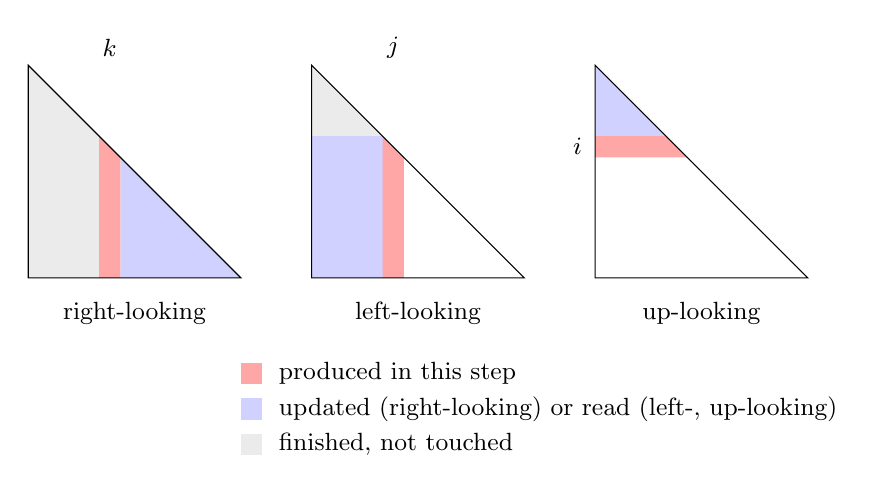
\begin{tikzpicture}[scale=0.9, every node/.style={font=\small}]
  \colorlet{prod}{red!35}
  \colorlet{touch}{blue!18}
  \colorlet{done}{black!8}
  % right-looking
  \begin{scope}
    \fill[done] (0,0) -- (1,-1) -- (1,-3) -- (0,-3) -- cycle;
    \fill[touch] (1.3,-1.3) -- (3,-3) -- (1.3,-3) -- cycle;
    \fill[prod] (1,-1) -- (1.3,-1.3) -- (1.3,-3) -- (1,-3) -- cycle;
    \draw (0,0) -- (3,-3) -- (0,-3) -- cycle;
    \node at (1.15,0.25) {$k$};
    \node at (1.5,-3.5) {right-looking};
  \end{scope}
  % left-looking
  \begin{scope}[xshift=4cm]
    \fill[done] (0,0) -- (1,-1) -- (0,-1) -- cycle;
    \fill[touch] (0,-1) rectangle (1,-3);
    \fill[prod] (1,-1) -- (1.3,-1.3) -- (1.3,-3) -- (1,-3) -- cycle;
    \draw (0,0) -- (3,-3) -- (0,-3) -- cycle;
    \node at (1.15,0.25) {$j$};
    \node at (1.5,-3.5) {left-looking};
  \end{scope}
  % up-looking
  \begin{scope}[xshift=8cm]
    \fill[touch] (0,0) -- (1,-1) -- (0,-1) -- cycle;
    \fill[prod] (0,-1) -- (1,-1) -- (1.3,-1.3) -- (0,-1.3) -- cycle;
    \draw (0,0) -- (3,-3) -- (0,-3) -- cycle;
    \node at (-0.25,-1.15) {$i$};
    \node at (1.5,-3.5) {up-looking};
  \end{scope}
  % legend
  \begin{scope}[yshift=-4.2cm, xshift=3cm]
    \fill[prod] (0,0) rectangle (0.3,-0.3); \node[anchor=west] at (0.4,-0.15) {produced in this step};
    \fill[touch] (0,-0.5) rectangle (0.3,-0.8); \node[anchor=west] at (0.4,-0.65) {updated (right-looking) or read (left-, up-looking)};
    \fill[done] (0,-1.0) rectangle (0.3,-1.3); \node[anchor=west] at (0.4,-1.15) {finished, not touched};
  \end{scope}
\end{tikzpicture}
\end{center}

\paragraph{Left-looking.} When column $j$ is reached, all updates that the finished columns to its left owe it are subtracted at once, and then the column is normalized. Right-looking pushes each finished column to the right immediately (\emph{eager}); left-looking pulls the updates in only when they are needed (\emph{lazy}). Each entry is written in its final form once, whereas in the right-looking variant the entries of the Schur complement are read and written $O(m)$ times. The innermost loop runs down a column, which suits column-major languages (Julia, Fortran, MATLAB).

\begin{algorithm}[H]
  \caption{Cholesky factorization, left-looking, in place (lower triangle).}
  \label{alg:chol-left}
  \begin{algorithmic}[1]
    \For{$j = 1, \dots, m$}
      \For{$k = 1, \dots, j - 1$}
        \For{$i = j, \dots, m$}
          \State $A_{ij} \gets A_{ij} - A_{ik}\overline{A_{jk}}$
        \EndFor
      \EndFor
      \State $s \gets \sqrt{A_{jj}}$ \Comment{save it: line 7 overwrites $A_{jj}$}
      \For{$i = j, \dots, m$}
        \State $A_{ij} \gets A_{ij} / s$
      \EndFor
    \EndFor
  \end{algorithmic}
\end{algorithm}

\paragraph{Up-looking.} The factor is computed row by row; row $i$ depends only on its own finished part and on the finished rows above. Row $i$ of $L$ is column $i$ of $R = L^\ast$, so in a column-major language one stores the upper triangular factor $R$ instead, and walking along a row of $L$ becomes walking down a column of $R$. In \emph{packed storage}, the upper triangle is stored column by column, column $i$ (of length $i$) right after column $i - 1$:
\begin{equation}
  \begin{bmatrix} 1 & 2 & 4 & 7 & 11 \\ & 3 & 5 & 8 & 12 \\ & & 6 & 9 & 13 \\ & & & 10 & 14 \\ & & & & 15 \end{bmatrix}.
\end{equation}
Computing column $i$ uses only earlier data, so when $A$ grows by one row and one column, the factor grows by appending one segment at the end.

\begin{algorithm}[H]
  \caption{Cholesky factorization, up-looking, in place (lower triangle).}
  \label{alg:chol-up}
  \begin{algorithmic}[1]
    \For{$i = 1, \dots, m$}
      \For{$j = 1, \dots, i$}
        \For{$k = 1, \dots, j - 1$}
          \State $A_{ij} \gets A_{ij} - A_{ik}\overline{A_{jk}}$
        \EndFor
        \If{$j < i$}
          \State $A_{ij} \gets A_{ij} / A_{jj}$ \Comment{$A_{jj}$ already holds $L_{jj}$}
        \Else
          \State $A_{ii} \gets \sqrt{A_{ii}}$
        \EndIf
      \EndFor
    \EndFor
  \end{algorithmic}
\end{algorithm}

\section{Existence of the Cholesky Factorization}
\label{sec:chol-exists}

LU without pivoting can meet a zero pivot; $\left[\begin{smallmatrix} 0 & 1 \\ 1 & 0 \end{smallmatrix}\right]$ fails at the very first step. Cholesky asks for more: the pivots must not only be nonzero but \emph{positive real numbers}, since we take their square roots. We first show that congruence preserves positive definiteness.

\begin{lemma}[Congruence Preserves Positive Definiteness]
  \label{lem:congruence}
  Let $A \in \K^{m \times m}$ be s.p.d.\ and $B \in \K^{m \times m}$ be nonsingular. Then $B^\ast AB$ is s.p.d.
\end{lemma}

\begin{proof}
  $B^\ast AB$ is Hermitian, since $(B^\ast AB)^\ast = B^\ast A^\ast B = B^\ast AB$. For positive definiteness, let $\vec{x} \ne \zerovec$. Since $B$ is nonsingular, $B\vec{x} \ne \zerovec$, and hence
  \begin{equation}
    \vec{x}^\ast B^\ast AB\vec{x} = (B\vec{x})^\ast A(B\vec{x}) > 0,
  \end{equation}
  as desired.
\end{proof}

If $B$ is singular, taking $\vec{x} \in \nullsp(B)$ gives $\vec{x}^\ast B^\ast AB\vec{x} = 0$, and we only get positive semidefiniteness.

\begin{theorem}[Existence of the Cholesky Factorization]
  \label{thm:chol-exists}
  Let $A \in \K^{m \times m}$ be s.p.d. Then Cholesky without pivoting encounters only positive real pivots $d_1, \dots, d_m$, and hence produces $A = LL^\ast$ with $L$ lower triangular with positive diagonal. Moreover, the pivots are bounded below by
  \begin{equation}
    \label{eq:pivot-bound}
    d_k \ge \frac{1}{\norm{A^{-1}}_2} = \lambda_{\min}(A), \qquad k = 1, \dots, m.
  \end{equation}
\end{theorem}

\begin{proof}
  We show by induction on $k$ that $d_{k+1}$ is a positive real number, $k = 0, \dots, m - 1$. Suppose that the first $k$ pivots are positive, so that the elimination matrices $L_1, \dots, L_k$ of the first $k$ steps are defined. (For $k = 0$ there is nothing to assume.) Each $L_i$ is unit lower triangular, and after $k$ symmetric steps,
  \begin{equation}
    S \doteq L_k \cdots L_1AL_1^\ast \cdots L_k^\ast = \begin{bmatrix} \diag(d_1, \dots, d_k) & 0 \\ 0 & S^{(k)} \end{bmatrix},
  \end{equation}
  where $S^{(k)}$ is the current Schur complement, whose top left entry is the next pivot $S_{k+1,k+1} = d_{k+1}$. Let $B = L_1^\ast \cdots L_k^\ast$, so that $B^\ast = L_k \cdots L_1$ and $S = B^\ast AB$. Each $L_i$ has determinant $1$, so $B$ is nonsingular, and by \Cref{lem:congruence} $S$ is s.p.d.

  The pivot is real: $S$ is Hermitian, so $S_{k+1,k+1} = \overline{S_{k+1,k+1}}$. The pivot is positive: the standard basis vector picks out a diagonal entry, $\vec{e}_j^\ast S\vec{e}_j = S_{jj}$, and by positive definiteness
  \begin{equation}
    d_{k+1} = S_{k+1,k+1} = \vec{e}_{k+1}^\ast S\vec{e}_{k+1} > 0.
  \end{equation}
  This completes the induction. With all pivots positive, the construction of the previous section gives $A = LL^\ast$ with $L_{kk} = \sqrt{d_k} > 0$. The lower bound \eqref{eq:pivot-bound} needs a lemma about Schur complements and is proved in \Cref{sec:schur}.
\end{proof}

The argument also shows a general fact: \emph{every diagonal entry of a positive definite matrix is positive}. Writing ``real'' and ``positive'' separately is deliberate: realness comes from the Hermitian property, positivity from definiteness. The lower bound says more than positivity: the pivots stay a fixed distance away from zero, independent of $k$, so small pivots cannot occur.

\begin{corollary}[Uniqueness of the Cholesky Factorization]
  \label{cor:chol-unique}
  An s.p.d.\ matrix has exactly one factorization $A = LL^\ast$ with $L$ lower triangular with positive diagonal.
\end{corollary}

\begin{proof}
  Existence is \Cref{thm:chol-exists}. Suppose $A = LL^\ast = MM^\ast$ with both factors of this form. Then $M^{-1}L = M^\ast L^{-\ast}$. The left side is lower triangular and the right side is upper triangular, so both equal a diagonal matrix $\Delta$, whose entries $L_{kk}/M_{kk}$ are positive. From $\Delta\Delta^\ast = M^{-1}LL^\ast M^{-\ast} = M^{-1}MM^\ast M^{-\ast} = I$ we get $\abs{\Delta_{kk}} = 1$, so $\Delta = I$ and $L = M$.
\end{proof}

\section{Rounding Errors}
\label{sec:chol-errors}

\subsection{The Key Quantity for LU}

By \Cref{thm:lu-backward}, the factors $\tilde{L}$, $\tilde{U}$ computed by LU satisfy $\tilde{L}\tilde{U} = A + \delta A$ with $\abs{\delta A} \le cm\epsm\abs{\tilde{L}}\abs{\tilde{U}}$ entrywise. The algorithm is stable when $\abs{L}\abs{U}$ is of the same size as $\abs{A}$, and errors are amplified when it is much larger. Without pivoting, $\abs{L}\abs{U}$ can be arbitrarily large: for $A = \left[\begin{smallmatrix} \delta & 1 \\ 1 & 1 \end{smallmatrix}\right]$ with small $\delta$, $L$ contains $1/\delta$.

\subsection{No Element Growth in Cholesky}

For Cholesky, $U = L^\ast$, and the key quantity is $\abs{L}\abs{L^\ast}$. We first need a fact about where the large entries of an s.p.d.\ matrix live.

\begin{lemma}[The Largest Entry Is on the Diagonal]
  \label{lem:spd-diag}
  Let $A$ be s.p.d. Then $\abs{A_{ij}} < \sqrt{A_{ii}A_{jj}}$ for all $i \ne j$. In particular, $\max_{i,j}\abs{A_{ij}} = \max_i A_{ii}$.
\end{lemma}

\begin{proof}
  Fix $i \ne j$. Applying positive definiteness to vectors supported on $\{i, j\}$ shows that the $2 \times 2$ principal submatrix $\left[\begin{smallmatrix} A_{ii} & A_{ij} \\ A_{ji} & A_{jj} \end{smallmatrix}\right]$ is s.p.d., so its eigenvalues are positive and so is its determinant: $A_{ii}A_{jj} - \abs{A_{ij}}^2 > 0$. Hence $\abs{A_{ij}} < \sqrt{A_{ii}A_{jj}} \le \max(A_{ii}, A_{jj})$.
\end{proof}

\begin{proposition}[No Growth in the Cholesky Factor]
  \label{prop:chol-growth}
  Let $A = LL^\ast$ be s.p.d. Then for all $i, j$,
  \begin{equation}
    \abs{L_{ij}} \le \sqrt{A_{ii}}, \qquad \left(\abs{L}\abs{L^\ast}\right)_{ij} \le \sqrt{A_{ii}A_{jj}} \le \max_{k,l}\abs{A_{kl}}.
  \end{equation}
\end{proposition}

\begin{proof}
  Comparing diagonal entries in $A = LL^\ast$ gives $A_{ii} = \sum_k\abs{L_{ik}}^2$, so $\abs{L_{ij}}^2 \le A_{ii}$. For the second claim, by the Cauchy--Schwarz inequality,
  \begin{equation}
    \left(\abs{L}\abs{L^\ast}\right)_{ij}
    = \sum_k\abs{L_{ik}}\abs{L_{jk}}
    \le \left(\sum_k\abs{L_{ik}}^2\right)^{1/2}\left(\sum_k\abs{L_{jk}}^2\right)^{1/2}
    = \sqrt{A_{ii}}\sqrt{A_{jj}}
    \le \max_{k,l}\abs{A_{kl}},
  \end{equation}
  where the last step uses \Cref{lem:spd-diag}.
\end{proof}

Here $\max_{k,l}\abs{A_{kl}} = \norm{\operatorname{vec}(A)}_\infty$ is the largest entry of $A$, where $\operatorname{vec}(A) \in \K^{m^2}$ stacks the columns of $A$; it is \emph{not} the induced $\infty$-norm (maximum row sum) of \Cref{prop:one-inf-norm}. In words, the growth factor of Cholesky is $1$. Substituting into the backward error bound gives the main result.

\begin{theorem}[Backward Stability of Cholesky]
  \label{thm:chol-stable}
  Let $A \in \K^{m \times m}$ be s.p.d., and suppose Cholesky runs to completion in floating-point arithmetic, producing $\tilde{L}$. Then, to first order in $\epsm$,
  \begin{equation}
    \tilde{L}\tilde{L}^\ast = A + \delta A, \qquad \abs{\delta A_{ij}} \le cm\epsm\max_{k,l}\abs{A_{kl}}
  \end{equation}
  for a modest constant $c$. That is, Cholesky without pivoting is backward stable.
\end{theorem}

\begin{proof}[Proof sketch]
  The analysis of \Cref{thm:lu-backward} applies with $\tilde{U} = \tilde{L}^\ast$ and gives $\abs{\delta A} \le cm\epsm\abs{\tilde{L}}\abs{\tilde{L}^\ast}$~\cite[Theorem 10.3]{Higham}. Strictly, \Cref{prop:chol-growth} applies to the exact factor; the computed one satisfies $\sum_k\abs{\tilde{L}_{ik}}^2 = A_{ii} + \delta A_{ii}$, which differs by a term of order $\epsm$ and changes the bound only at second order. Hence $\abs{\tilde{L}}\abs{\tilde{L}^\ast} \le \max_{k,l}\abs{A_{kl}}$ to first order, as desired.
\end{proof}

\Cref{thm:chol-exists,thm:chol-stable} answer two different questions. The existence theorem guarantees that the algorithm runs to completion in exact arithmetic; the stability theorem guarantees that in floating point it computes accurately. Pivoting in LU is there to fix both at once; for s.p.d.\ matrices both hold automatically. (In floating point, completion itself is guaranteed as long as $\kappa_2(A)$ is not too close to $1/\epsm$~\cite[Theorem 10.7]{Higham}.)

\subsection{Symmetric Indefinite Matrices}

A Hermitian matrix is \emph{indefinite} if $\vec{x}^\ast A\vec{x}$ takes both positive and negative values, equivalently if it has both positive and negative eigenvalues. For such matrices one computes
\begin{equation}
  PAP^\T = LDL^\T,
\end{equation}
where $P$ is a permutation and $D$ is block diagonal with $1 \times 1$ and $2 \times 2$ blocks ($LDL^\ast$ in the complex case). The symmetric permutation $PAP^\T$ swaps rows and columns in the same way, so it preserves symmetry and we can still work on one half; the ordinary $PA$ swaps only rows and destroys symmetry. But a symmetric permutation only moves diagonal entries to other diagonal positions; it cannot bring an off-diagonal entry onto the diagonal. For example,
\begin{equation}
  A = \begin{bmatrix} 0 & 1 \\ 1 & 0 \end{bmatrix}
\end{equation}
has only zeros on the diagonal, so every $1 \times 1$ pivot is zero no matter how we permute. The way out is to take the whole $2 \times 2$ block as a single pivot: it is invertible, so it becomes one block of $D$ with $L = I$.

In general, each step moves an invertible $1 \times 1$ or $2 \times 2$ block $E$ to the top left and factors
\begin{equation}
  PAP^\T = \begin{bmatrix} E & C^\ast \\ C & B \end{bmatrix} = \begin{bmatrix} I & 0 \\ CE^{-1} & I \end{bmatrix}\begin{bmatrix} E & 0 \\ 0 & B - CE^{-1}C^\ast \end{bmatrix}\begin{bmatrix} I & E^{-1}C^\ast \\ 0 & I \end{bmatrix},
\end{equation}
and then recurses on the Schur complement, exactly as in the derivation of Cholesky. The practical rule for choosing the blocks is \emph{Bunch--Kaufman pivoting} (LAPACK \texttt{sytrf}): when a diagonal entry is too small relative to the off-diagonal entries in its column, a $2 \times 2$ block is used instead, which avoids small pivots. Its stability is on the level of LU with partial pivoting, and it costs about $\frac{1}{3}m^3$ flops.

\section{Schur Complements}
\label{sec:schur}

\subsection{Block Cholesky}

Partition $A = LL^\ast$ into $2 \times 2$ blocks, with $L_{11}$ and $L_{22}$ square lower triangular:
\begin{equation}
  L = \begin{bmatrix} L_{11} & 0 \\ L_{21} & L_{22} \end{bmatrix}, \qquad
  A = \begin{bmatrix} A_{11} & A_{12} \\ A_{21} & A_{22} \end{bmatrix}, \qquad
  LL^\ast = \begin{bmatrix} L_{11}L_{11}^\ast & L_{11}L_{21}^\ast \\ L_{21}L_{11}^\ast & L_{21}L_{21}^\ast + L_{22}L_{22}^\ast \end{bmatrix}.
\end{equation}
Comparing blocks,
\begin{equation}
  L_{11}L_{11}^\ast = A_{11}, \qquad L_{21}L_{11}^\ast = A_{21}, \qquad L_{21}L_{21}^\ast + L_{22}L_{22}^\ast = A_{22};
\end{equation}
the top right block is the conjugate transpose of the second equation and gives nothing new. The second equation gives $L_{21} = A_{21}L_{11}^{-\ast}$, so, using $A_{21}^\ast = A_{12}$,
\begin{equation}
  L_{21}L_{21}^\ast = A_{21}L_{11}^{-\ast}L_{11}^{-1}A_{21}^\ast = A_{21}(L_{11}L_{11}^\ast)^{-1}A_{21}^\ast = A_{21}A_{11}^{-1}A_{12}.
\end{equation}
Substituting into the third equation,
\begin{equation}
  L_{22}L_{22}^\ast = A_{22} - A_{21}A_{11}^{-1}A_{12}.
\end{equation}

\begin{definition}[Schur Complement]
  Let $A = \left[\begin{smallmatrix} A_{11} & A_{12} \\ A_{21} & A_{22} \end{smallmatrix}\right]$ with $A_{11}$ square and invertible. The \emph{Schur complement} of $A_{11}$ in $A$ is
  \begin{equation}
    A/A_{11} \doteq A_{22} - A_{21}A_{11}^{-1}A_{12}.
  \end{equation}
\end{definition}

The elimination of the previous sections is the special case of a $1 \times 1$ block $A_{11} = \alpha$, where $A_{11}^{-1}$ is division by a scalar. Strictly speaking, the Schur complement is $A_{22} - A_{21}A_{11}^{-1}A_{12}$, which happens to equal $L_{22}L_{22}^\ast$. The block equations say two things. First, $L_{22}$ is the Cholesky factor of the Schur complement, so the algorithm can recurse on blocks. Second, the Schur complement equals $L_{22}L_{22}^\ast$ with $L_{22}$ invertible, so it is s.p.d.; this is a second proof, besides the congruence argument, that the recursion never breaks down.

\subsection{The Inverse and the Schur Complement}

\begin{lemma}[Blocks of the Inverse]
  \label{lem:schur-inverse}
  Let $A = \left[\begin{smallmatrix} A_{11} & A_{12} \\ A_{21} & A_{22} \end{smallmatrix}\right]$ be invertible with $A_{11}$ invertible, let $S = A_{22} - A_{21}A_{11}^{-1}A_{12}$ be invertible, and partition $\Theta \doteq A^{-1}$ in the same way. Then
  \begin{equation}
    \Theta_{22} = S^{-1}.
  \end{equation}
\end{lemma}

\begin{proof}
  Block elimination gives
  \begin{equation}
    A = \begin{bmatrix} I & 0 \\ A_{21}A_{11}^{-1} & I \end{bmatrix}\begin{bmatrix} A_{11} & 0 \\ 0 & S \end{bmatrix}\begin{bmatrix} I & A_{11}^{-1}A_{12} \\ 0 & I \end{bmatrix}.
  \end{equation}
  A unit block triangular matrix is inverted by negating its off-diagonal block, so
  \begin{equation}
    A^{-1} = \begin{bmatrix} I & -A_{11}^{-1}A_{12} \\ 0 & I \end{bmatrix}\begin{bmatrix} A_{11}^{-1} & 0 \\ 0 & S^{-1} \end{bmatrix}\begin{bmatrix} I & 0 \\ -A_{21}A_{11}^{-1} & I \end{bmatrix}.
  \end{equation}
  The second block row of the left factor is $\begin{bmatrix} 0 & I \end{bmatrix}$ and the second block column of the right factor is $\begin{bmatrix} 0 & I \end{bmatrix}^\T$, so the lower right block of the product is $S^{-1}$.
\end{proof}

The proof uses only that $A_{11}$ and $S$ are invertible; neither symmetry nor definiteness is needed.

\subsection{Proof of the Pivot Bound}

We now prove \eqref{eq:pivot-bound}.

\begin{proof}[Proof of \eqref{eq:pivot-bound}]
  Fix $k$, and let $S'$ be the Schur complement of the leading $(k - 1) \times (k - 1)$ block of $A$ (for $k = 1$, $S' = A$). By the block elimination above, $S'$ is the matrix left over after $k - 1$ steps, so the $k$-th pivot is its top left entry, $d_k = \vec{e}_1^\ast S'\vec{e}_1$. By \Cref{lem:schur-inverse}, $(S')^{-1} = \Theta[k{:}m, k{:}m]$ is a principal submatrix of $A^{-1}$. A submatrix has no larger $2$-norm than the whole matrix (it is $P^\T\Theta P$ for a matrix $P$ with orthonormal columns), so
  \begin{equation}
    \norm{(S')^{-1}}_2 \le \norm{A^{-1}}_2.
  \end{equation}
  Since $S'$ is s.p.d., its singular values are its eigenvalues, and $\norm{(S')^{-1}}_2 = 1/\lambda_{\min}(S')$ by \Cref{thm:twonorm}. Therefore
  \begin{equation}
    d_k = \vec{e}_1^\ast S'\vec{e}_1 \ge \lambda_{\min}(S') = \frac{1}{\norm{(S')^{-1}}_2} \ge \frac{1}{\norm{A^{-1}}_2},
  \end{equation}
  where the first inequality is the Rayleigh quotient bound $\vec{x}^\ast S'\vec{x} \ge \lambda_{\min}(S')\norm{\vec{x}}^2$. Finally $1/\norm{A^{-1}}_2 = \lambda_{\min}(A)$, again because $A$ is s.p.d.
\end{proof}

\section{(SUPPLEMENT) Further Topics}

\paragraph{The roles of symmetry and definiteness.} Both conditions are needed, but they do different jobs. Symmetry lets the row and the column eliminations share the same multipliers, which produces the shape $LDL^\ast$. Definiteness makes every pivot positive (no pivoting needed), keeps the recursion going (every Schur complement is again positive definite), allows the square root at the end, and brings stability.

\begin{center}
\begin{tabular}{p{0.3\textwidth}p{0.62\textwidth}}
  \toprule
  Case & Outcome \\
  \midrule
  symmetric, positive definite & Cholesky $A = R^\ast R$, no pivoting, stable \\
  symmetric, indefinite & pivots may vanish; even if $LDL^\ast$ exists, $D$ has negative entries; use Bunch--Kaufman \\
  positive definite, not symmetric (real) & pivots still positive and LU without pivoting completes, but no $R^\ast R$ \\
  symmetric positive semidefinite & pivots may vanish; $R^\ast R$ exists but is not unique; use pivoted Cholesky \\
  \bottomrule
\end{tabular}
\end{center}

In the semidefinite case, $A_{11} = 0$ forces the whole first row and column to vanish (the argument of \Cref{lem:spd-diag}, applied to a semidefinite matrix, gives $\abs{A_{1j}}^2 \le A_{11}A_{jj}$), so that step can simply be skipped.

\paragraph{Over $\R$, ``positive definite'' does not imply symmetric.} Starting from $A = B^\ast B$, a real $A$ is automatically symmetric. But if we only ask that $\vec{x}^\T A\vec{x} > 0$ for all real $\vec{x} \ne \zerovec$, then $A$ need not be symmetric: for example, $A = \left[\begin{smallmatrix} 1 & 1 \\ -1 & 1 \end{smallmatrix}\right]$ has $\vec{x}^\T A\vec{x} = x_1^2 + x_2^2$. Every real square matrix is the sum of a symmetric and a skew-symmetric part, and the skew-symmetric part $K$ has $\vec{x}^\T K\vec{x} = 0$, so the quadratic form only sees the symmetric part. This is why, over $\R$, symmetry is stated as a separate condition in ``s.p.d.''. Over $\C$ it is automatic: if $\vec{x}^\ast A\vec{x}$ is real for all complex $\vec{x}$, then $\vec{x}^\ast(A - A^\ast)\vec{x} = 0$ for all $\vec{x}$, and substituting $\vec{x} = \vec{e}_j + \vec{e}_k$ and $\vec{x} = \vec{e}_j + i\vec{e}_k$ (polarization) gives $A = A^\ast$. The example above, at $\vec{x} = (1, i)^\T$, gives $2 - 2i$, so it is not positive definite over $\C$.

\paragraph{Positive definiteness is necessary for Cholesky.} If $A = R^\ast R$ with $R$ invertible, then $\vec{x}^\ast A\vec{x} = \norm{R\vec{x}}^2 > 0$ for $\vec{x} \ne \zerovec$, so $A$ must be positive definite. When $A$ is not positive definite, the algorithm is not failing for lack of cleverness: the factorization it seeks does not exist. Moreover, unit lower triangular congruences do not change the determinants of the leading principal submatrices, so $\det A[1{:}k, 1{:}k] = d_1 \cdots d_k$, and the pivots are ratios of consecutive leading principal minors,
\begin{equation}
  d_k = \frac{\det A[1{:}k, 1{:}k]}{\det A[1{:}k-1, 1{:}k-1]}.
\end{equation}
Combined with Sylvester's criterion (a Hermitian matrix is positive definite if and only if all its leading principal minors are positive),
\begin{equation}
  \begin{aligned}
    A \text{ is positive definite} &\iff \text{all leading principal minors are} > 0 \\
    &\iff \text{all pivots are} > 0 \iff \text{Cholesky completes}.
  \end{aligned}
\end{equation}
Cholesky is therefore the standard test for positive definiteness, much cheaper than computing eigenvalues; \texttt{numpy.linalg.cholesky} raises \texttt{LinAlgError} on a non-positive-definite input exactly at this point.

\paragraph{Pivots are not eigenvalues.} The diagonal entries of $D$ in $A = \tilde{L}D\tilde{L}^\ast$ are the pivots, which in general differ from the eigenvalues. For example, $\left[\begin{smallmatrix} 2 & 1 \\ 1 & 2 \end{smallmatrix}\right]$ has eigenvalues $1, 3$ and pivots $2, \frac{3}{2}$; only the products agree, both equal to $\det A = 3$. The reason is that $\tilde{L}^\ast \ne \tilde{L}^{-1}$: this is a \emph{congruence}, not a similarity (compare $A = Q\Lambda Q^\ast$ with $Q^\ast = Q^{-1}$). What a congruence preserves is the \emph{inertia} (Sylvester's law of inertia): the numbers of positive, negative, and zero eigenvalues. So the number of positive pivots equals the number of positive eigenvalues. For instance, $\left[\begin{smallmatrix} 1 & 2 \\ 2 & 1 \end{smallmatrix}\right]$ has eigenvalues $3, -1$ and pivots $1, -3$: different values, but one positive and one negative each. The equivalence ``all pivots $> 0 \iff$ positive definite'' rests on exactly this, and the block diagonal $D$ of Bunch--Kaufman reveals the inertia of $A$ in the same way.

\paragraph{Definiteness at a glance.} ``Definite'' means that the sign is determined. A Hermitian matrix is positive (semi)definite if $\vec{x}^\ast A\vec{x} > 0$ ($\ge 0$) for all $\vec{x} \ne \zerovec$, equivalently all eigenvalues are $> 0$ ($\ge 0$); negative (semi)definite is defined likewise; and it is indefinite if $\vec{x}^\ast A\vec{x}$ takes both signs, equivalently there are both positive and negative eigenvalues. For example, $\left[\begin{smallmatrix} 0 & 1 \\ 1 & 0 \end{smallmatrix}\right]$ has the quadratic form $2x_1x_2$, positive along $(1, 1)$ and negative along $(1, -1)$: its graph is a saddle. In optimization, an indefinite Hessian signals a saddle point. A matrix with eigenvalues $1, 0, -1$ is also indefinite.

\paragraph{Blocked Cholesky and hardware.} Libraries (LAPACK and cuSOLVER \texttt{potrf}) use a blocked version, as for LU in \Cref{sec:blocked-lu}. Take $A_{11}$ to be a block of size, say, $256 \times 256$ and factor it; then $L_{21} = A_{21}L_{11}^{-\ast}$ is a triangular solve with many right-hand sides (TRSM), and the Schur complement update $A_{22} - L_{21}L_{21}^\ast$ is a matrix multiplication (SYRK/GEMM). Almost all flops land in Level 3 BLAS and run close to peak. This continues the discussion of memory access in the left- and up-looking variants.

\paragraph{A statistical interpretation.} If $A$ is the covariance matrix of a Gaussian vector $(\vec{x}_1, \vec{x}_2)$, then the Schur complement $A_{22} - A_{21}A_{11}^{-1}A_{12}$ is exactly the conditional covariance of $\vec{x}_2$ given $\vec{x}_1$. \Cref{lem:schur-inverse} then says that the corresponding block of the precision matrix $A^{-1}$ is the inverse of the conditional covariance. Much of sparse Cholesky for Gaussian processes and kernel methods builds on this correspondence.

\paragraph{The normal equations, again.} Backward stability of Cholesky means that the computed $\tilde{R}$ is the exact Cholesky factor of $A^\ast A + \delta$ with a small $\delta$. When least squares is solved through the normal equations, however, the matrix being factored is $A^\ast A$, and the error in $\vec{x}$ is amplified by $\kappa(A^\ast A) = \kappa(A)^2$. So a stable Cholesky does not make ``normal equations plus Cholesky'' a stable least squares solver; for ill-conditioned $A$, QR is still the method of choice (\Cref{ch:normal}).
